\documentclass[compress, 10pt]{beamer}

% defining colors that can be used -----------------------------------------

% FRANKLIN AND MARSHALL COLLEGE COLORS
\definecolor{fandm01col}{HTML}{003B70} % PMS 541
\definecolor{fandm02col}{HTML}{00C0F2} % cyan
\definecolor{fandm03col}{HTML}{91C6DF} % light blue
\definecolor{fandm04col}{HTML}{009CC1} % teal
\definecolor{fandm05col}{HTML}{4873A2} % periwinkle
\definecolor{fandm06col}{HTML}{0035AD} % PMS 286

% DARK MODE COLORS (FROM APPLE WEBSITE)
\definecolor{dark01col}{RGB}{242, 242, 247} % level 1 (white)
\definecolor{dark02col}{RGB}{142, 142, 147} % level 2
\definecolor{dark03col}{RGB}{99, 99, 102}   % level 3
\definecolor{dark04col}{RGB}{72, 72, 74}    % level 4
\definecolor{dark05col}{RGB}{44, 44, 46}    % level 5 (background)
\definecolor{dark06col}{RGB}{28, 28, 30}    % level 6 

% BASE COLORS (FROM APPLE WEBSITE)
\definecolor{app01col}{RGB}{10, 132, 255} % blue
\definecolor{app02col}{RGB}{48, 209, 88}  % green
\definecolor{app03col}{RGB}{255, 159, 10} % orange
\definecolor{app04col}{RGB}{255, 55, 95}  % pink
\definecolor{app05col}{RGB}{191, 90, 242} % purple

% COLOR BLIND COLORS
\definecolor{mycol01}{HTML}{E69F00} % orange
\definecolor{mycol02}{HTML}{56B4E9} % blue
\definecolor{mycol03}{HTML}{009E73} % green
\definecolor{mycol04}{HTML}{F0E442} % yellow
\definecolor{mycol05}{HTML}{CC79A7} % pink

% customizing the theme of the slides --------------------------------------

%\usetheme{Luebeck}

\usecolortheme[named=fandm03col]{structure} % 3-5 look good
%\usecolortheme{sidebartab}
\useinnertheme{circles} % changes style of itemized/enumerate stuff
\useoutertheme{default}


\setbeamertemplate{navigation symbols}{}
%

\usefonttheme{serif}

%\usepackage[scaled]{helvet}
%\renewcommand\familydefault{\sfdefault}
%\usepackage[T1]{fontenc}

\renewcommand\mathfamilydefault{\rmdefault} % changing the math font to serif

%\setbeamertemplate{footline}[frame number]{}
%\setbeamertemplate{navigation symbols}{} % getting rid of the navigation bar

\setbeamercolor{background canvas}{bg = dark05col} % making background dark
\setbeamercolor{normal text}{fg = dark01col} % making base text white



% defining custom commands
\newcommand{\mydef}[1]{\textcolor{mycol04}{\textit{#1}}}
\newcommand<>{\myhil}[1]{\textcolor#2{mycol01}{#1}}
\newcommand<>{\myhila}[2]{\textcolor#3{#2}{#1}}
\newcommand<>{\mydark}[1]{\textcolor#2{dark03col}{#1}}
\newcommand{\myskip}{\vspace{-1.5em}}



\setlength{\parskip}{2em}

\usepackage{bm}



%%%%%%%%%%%%%%%%%%%%%%%%%%%%%%%%%%%%%%%%%%%%%%%%%%%%%%%%%%%%%%%%%%%%%%%%%%%%%%%%%%%%%%%%
%%%%%%%%%%%%%%%%%%%%%%%%%%%%%%%%%%%%%%%%%%%%%%%%%%%%%%%%%%%%%%%%%%%%%%%%%%%%%%%%%%%%%%%%
%%%%%%%%%%%%%%%%%%%%%%%%%%%%%%%%%%%%%%%%%%%%%%%%%%%%%%%%%%%%%%%%%%%%%%%%%%%%%%%%%%%%%%%%



\title{Modeling Epidemics and the Effect of Social Distancing}
\author{Aiden Kenny}
\institute{Franklin \&{} Marshall College}
\date{April 30, 2020}



\begin{document}



\begin{frame}

\maketitle
    
\end{frame}



\begin{frame}{Some background}

\onslide<1->{
An \mydef{infectious disease} is a clinically evident illness resulting from the presence of a pathogenic microbial agent.
}

\myskip
\begin{itemize}
    \item<2-> e.g. HIV, smallpox, COVID-19
\end{itemize}

\onslide<3->{
An \mydef{epidemic} is an unusually large, short-term (less than a year) outbreak of a disease.
}

\onslide<4->{
We are interested in modeling the progress of these infectious diseases as they spread through the population during an epidemic.
}
    
\end{frame}



\begin{frame}{Compartmental models}

\onslide<1->{
We can split the population into several \mydef{compartments}, or groups. 
}

\onslide<2->{
These compartments describe the individuals' relationship to the infectious disease.
} 

\myskip
\begin{itemize}
    \item<3-> e.g. Individuals who are currently infected. 
\end{itemize}

\onslide<4->{
People move between compartments as the epidemic progresses.
}

\myskip
\begin{itemize}
    \item<5-> e.g. People who are infected can get better.
\end{itemize}

\onslide<6->{
\mydef{Compartmental models} describe how the population moves through the compartments.
}
    
\end{frame}



\begin{frame}{More on compartments}

\onslide<1->{
A very simple model breaks the population into \textit{three} compartments:
}

\myskip
\begin{itemize}
    \item<1-> \myhila<2>{\textbf{S}}{mycol04} : individuals who are \myhila<2>{susceptible}{mycol04} to the disease.
    \item<1-> \myhila<3>{\textbf{I}}{mycol04} : individuals who are \myhila<3>{infected}{mycol04} with the disease.
    \item<1-> \myhila<4>{\textbf{R}}{mycol04} : individuals who are \myhila<4>{removed}{mycol04} and can no longer be infected.
\end{itemize}

\onslide<5->{
$S \ge 0$, $I \ge 0$, and $R \ge 0$ for all time $t \ge 0$.
}

\onslide<6->{
Let $N$ denote the total population at a given time $t \ge 0$.
}

\onslide<7->{
We have the general relationship 
\begin{align*}
    N(t) = S(t) + I(t) + R(t)
\end{align*}
for all $t \ge 0$. 
}
    
\end{frame}



\begin{frame}{The SIR model}

\onslide<1->{
\myhila<2-3>{A very basic system of differential equations that models these compartments is the \myhila<1>{\textit{SIR model}}{mycol04},
\begin{align*}
    \frac{\mathrm{d}S}{\mathrm{d}t} &= - \frac{\myhila<2>{\beta}{mycol04} SI}{N} \\[1.5ex]
    \frac{\mathrm{d}I}{\mathrm{d}t} &= \frac{\myhila<2>{\beta}{mycol04} SI}{N} - \myhila<3>{\gamma}{mycol04} I \\[1.5ex]
    \frac{\mathrm{d}R}{\mathrm{d}t} &= \myhila<3>{\gamma}{mycol04} I. \\
\end{align*}}{dark02col}
}

\myskip\myskip
\onslide<2->{
\myhila<3>{\myhila<2>{$\beta$}{mycol04} is known as the \myhila<2>{\textit<2>{infection rate}}{mycol04}.}{dark02col}
}

\myskip
\onslide<3->{
\myhila<3>{$\bm{\gamma}$}{mycol04} is known as the \myhila<3>{\textit<3>{healing rate}}.
}

\myskip
\onslide<4->{
$\beta > 0$ and $\gamma > 0$. 
}
    
\end{frame}



\begin{frame}{Some assumptions}

\onslide<1->{
\mydark<8>{We make several assumptions for our model:}
}

\myskip
\begin{itemize}
    \item<2-> \mydark<8>{The population is large $\to$ can be treated as continuous.}
    \item<3-> \mydark<8>{The population is a \textit{constant} number $N$.}
    \item<4-> \mydark<8>{Epidemic $\to$ no vital dynamic (no births or deaths).}
    \item<5-> \mydark<8>{Once removed, an individual \textit{cannot} contract the disease again.}
    \item<6-> Individuals do not change their behavior as epidemic progresses.
\end{itemize}

\onslide<7->{
\myhila<8>{The SIR model, with all these assumptions, can be a building block for more sophisticated models.}{dark03col}
}

\onslide<8->{
Namely, we can account for how \mydef{social distancing} effects the progression of an epidemic.
}

\end{frame}



\begin{frame}{Initial conditions}

\onslide<1->{
Let $S(0) = S_0$ and $I(0) = I_0$ be the values of $S$ and $I$ at $t = 0$. 
}

\onslide<2->{
We assume that $R(0) = 0$, meaning:
\myskip
\begin{itemize}
    \item No one is removed from the epidemic at $t = 0$.
    \item $S_0 + I_0 = N$.
\end{itemize}
}

\onslide<3->{
We also assume that $S_0 \approx N$, meaning:
\myskip
\begin{itemize}
    \item Most of the population is initially susceptible at $t = 0$.
    \item One a small number of individuals are infected at $t = 0$.
\end{itemize}
}
    
\end{frame}



\begin{frame}{Nullclines and equilibria}

\onslide<1->{
Notice that neither $\mathrm{d}S/\mathrm{d}t$ nor $\mathrm{d}I/\mathrm{d}t$ depend on $R$.
}

\myskip
\begin{itemize}
    \item<2-> $R$ has no effect on the equilibrium points.
    \item<2-> We can analyze the phase portrait of the $S$-$I$ plane.
\end{itemize}

\onslide<3->{
Since $S + I + R = N$ and $R \ge 0$, we have $S + I \le N$ as the region of possible values.
\myskip
\begin{itemize}
    \item Remember that we will start on the line $S + I = N$.
\end{itemize}
}

\onslide<4->{
Setting $\mathrm{d}S/\mathrm{d}t = 0$ gives us \myhila<4>{$S = 0$}{mycol04} or \myhila<4>{$I = 0$}{mycol04} as the two $S$-nullclines. 
}

\onslide<5->{
We can see that \myhila<5>{$\mathrm{d}S/\mathrm{d}t < 0$}{mycol04} for all values of $t$, so the number of susceptible individuals is \textit{always decreasing}.
}
    
\end{frame}



\begin{frame}{}

\only<1-2>{
\mydark<2>{We have
\begin{align*}
    \frac{\mathrm{d}I}{\mathrm{d}t} = \frac{\beta S I}{N} - \gamma I = \gamma I \left(\myhila<2>{\frac{\beta}{\gamma}}{mycol04} \frac{S}{N} - 1  \right).
\end{align*}}
}

\only<3->{
\mydark<3>{We have
\begin{align*}
    \frac{\mathrm{d}I}{\mathrm{d}t} = \frac{\beta S I}{N} - \gamma I = \gamma I \left(\myhila<3>{\mathcal{R}_0}{mycol04} \frac{S}{N} - 1  \right).
\end{align*}}
}

\myskip
\onslide<2->{
The coefficient \myhila<2>{$\beta/\gamma$}{mycol04} is called the \mydef{basic reproduction number}.
}

\myskip
\begin{itemize}
    \item<3-> It is denoted as \myhila<3>{$\mathcal{R}_0$}{mycol04}.
\end{itemize}

\onslide<4->{
Setting $\mathrm{d}I/\mathrm{d}t = 0$ gives us \myhila<4>{$I = 0$}{mycol04} and \myhila<4>{$S = N/\mathcal{R}_0$}{mycol04} as the two $I$-nullclines.
}

\onslide<5->{
The value of $\mathcal{R}_0$ effects the severity of the epidemic.
}
    
\end{frame}



\begin{frame}{Phase portrait}

\onslide<1->{
We conclude that everywhere on the line \myhila<1>{$I = 0$}{mycol04} is an equilibrium point.
}

\begin{figure}
    \centering
    \onslide<2->{
\includegraphics[width = 0.45\textwidth]{images/blank.png}} \hfill
    \onslide<3->{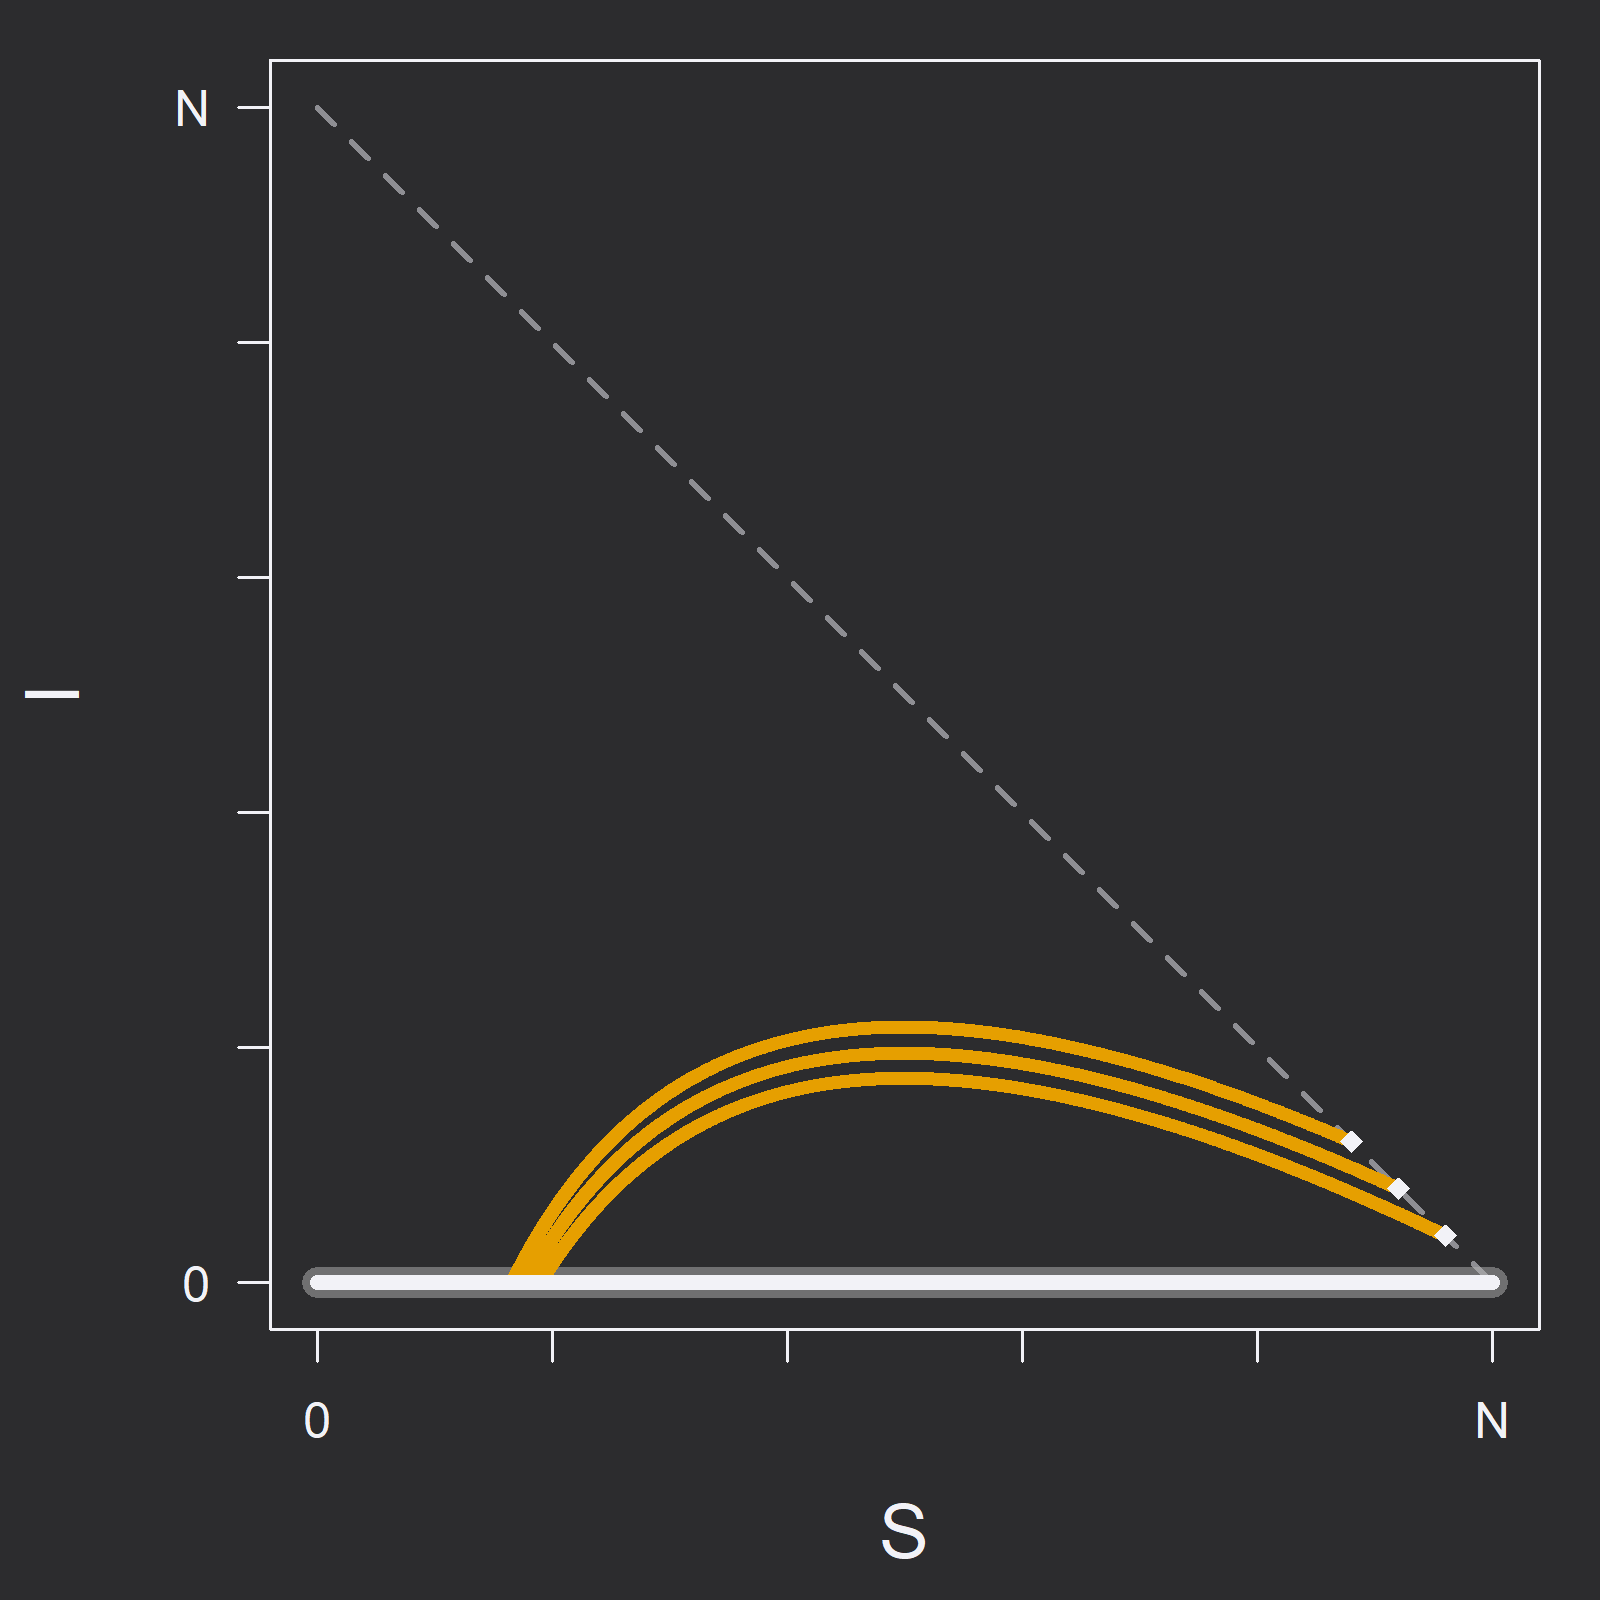
\includegraphics[width = 0.45\textwidth]{images/basic.png}}
\end{figure}
    
\end{frame}



\begin{frame}{Effect of $\mathcal{R}_0$}

\onslide<1->{
\mydark<7>{We see two things from the previous slides:}
}

\myskip
\begin{itemize}
    \item<2-> \mydark<7>{If $S > N/\mathcal{R}_0$, then $\mathrm{d}I/\mathrm{d}t > 0$.}
    \item<3-> If $S < N/\mathcal{R}_0$, then $\mathrm{d}I/\mathrm{d}t < 0$.
\end{itemize}

\onslide<4-> \mydark<7>{At the point $S_p = N / \mathcal{R}_0$, we have the \myhila<4>{\textit<4>{maximum}}{mycol04} number of infected.}

\onslide<5->{
Note: if $\mathcal{R}_0 < 1$, then we have $S_p > N$.
}

\myskip
\begin{itemize}
    \item<6-> The peak is located \myhila<6>{\textit<6>{outside}}{mycol04} of the possible values of $S$.
    \item<7-> Will \myhila<7>{\textit<7>{always}}{mycol04} have $S < N / \mathcal{R}_0$ $\to$ will \myhila<7>{\textit<7>{always}}{mycol04} have $\mathrm{d}I/\mathrm{d}t < 0$.
\end{itemize}
    
\end{frame}



\begin{frame}{}

\begin{figure}
    \centering
    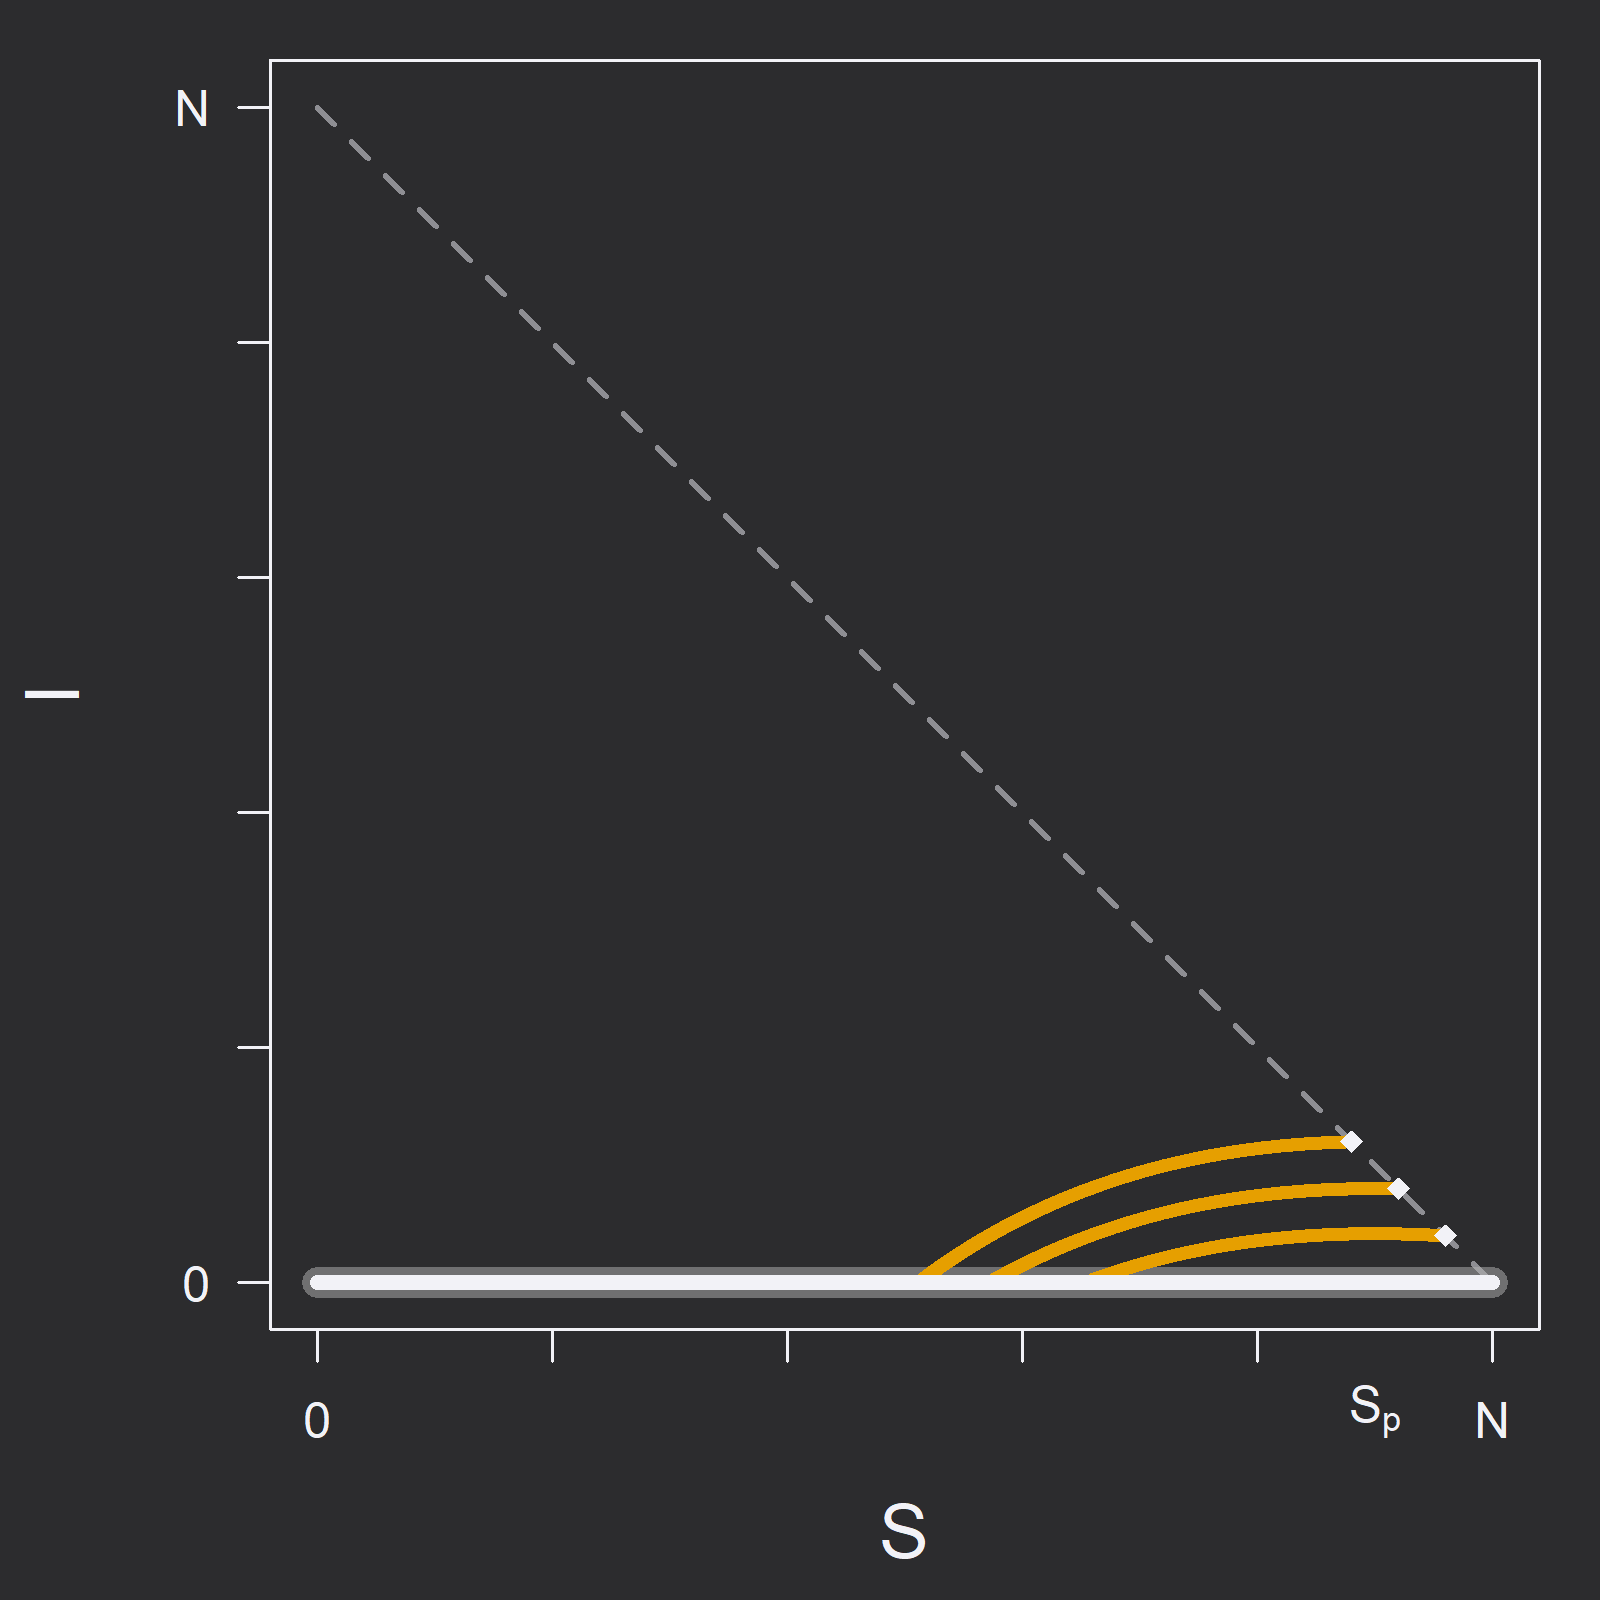
\includegraphics[width = 0.32\textwidth]{images/peak06.png} \hfill
    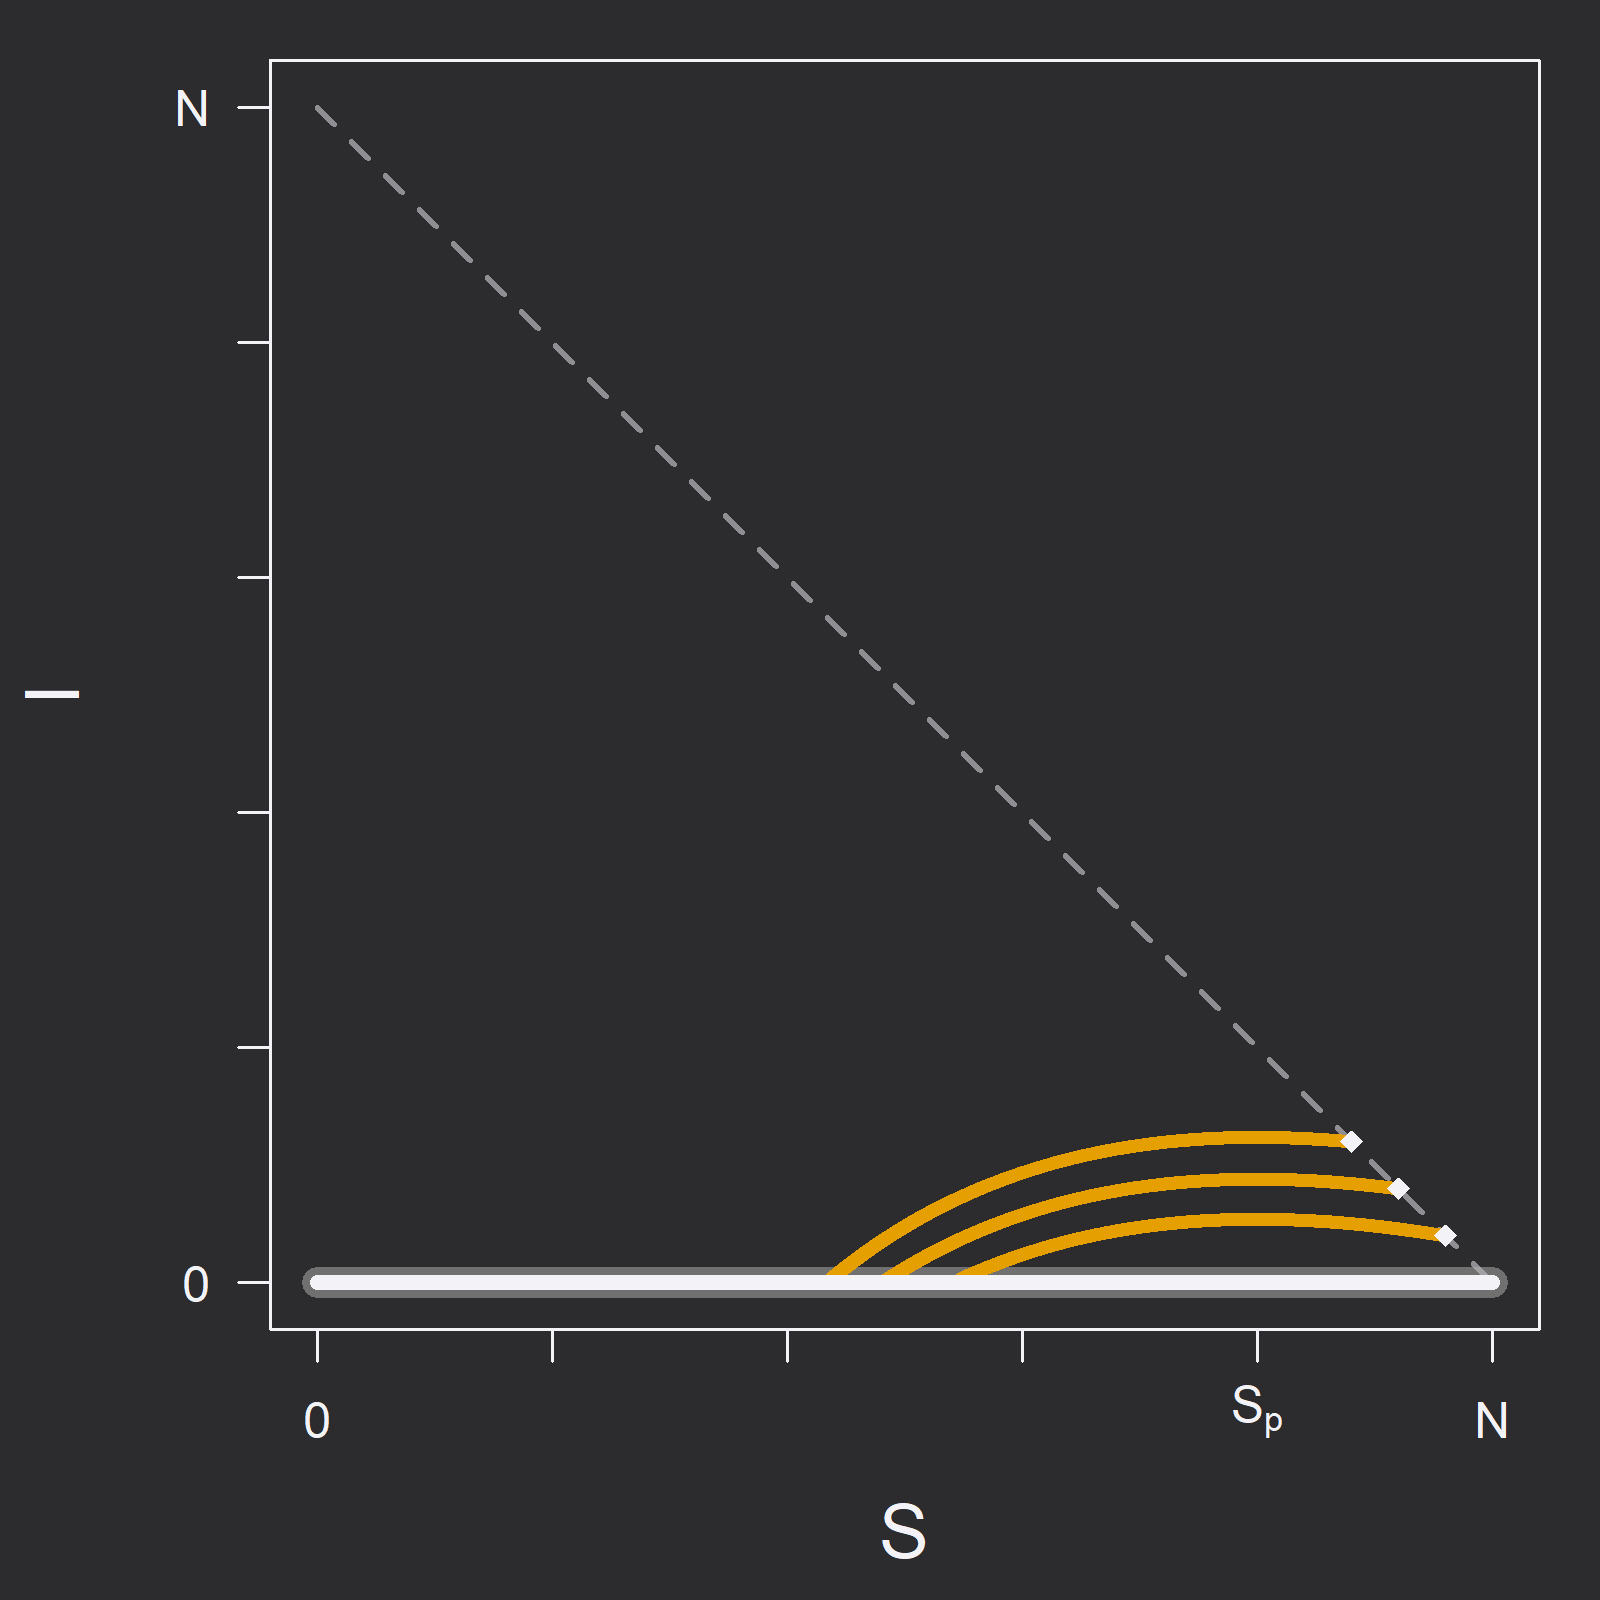
\includegraphics[width = 0.32\textwidth]{images/peak05.png} \hfill
    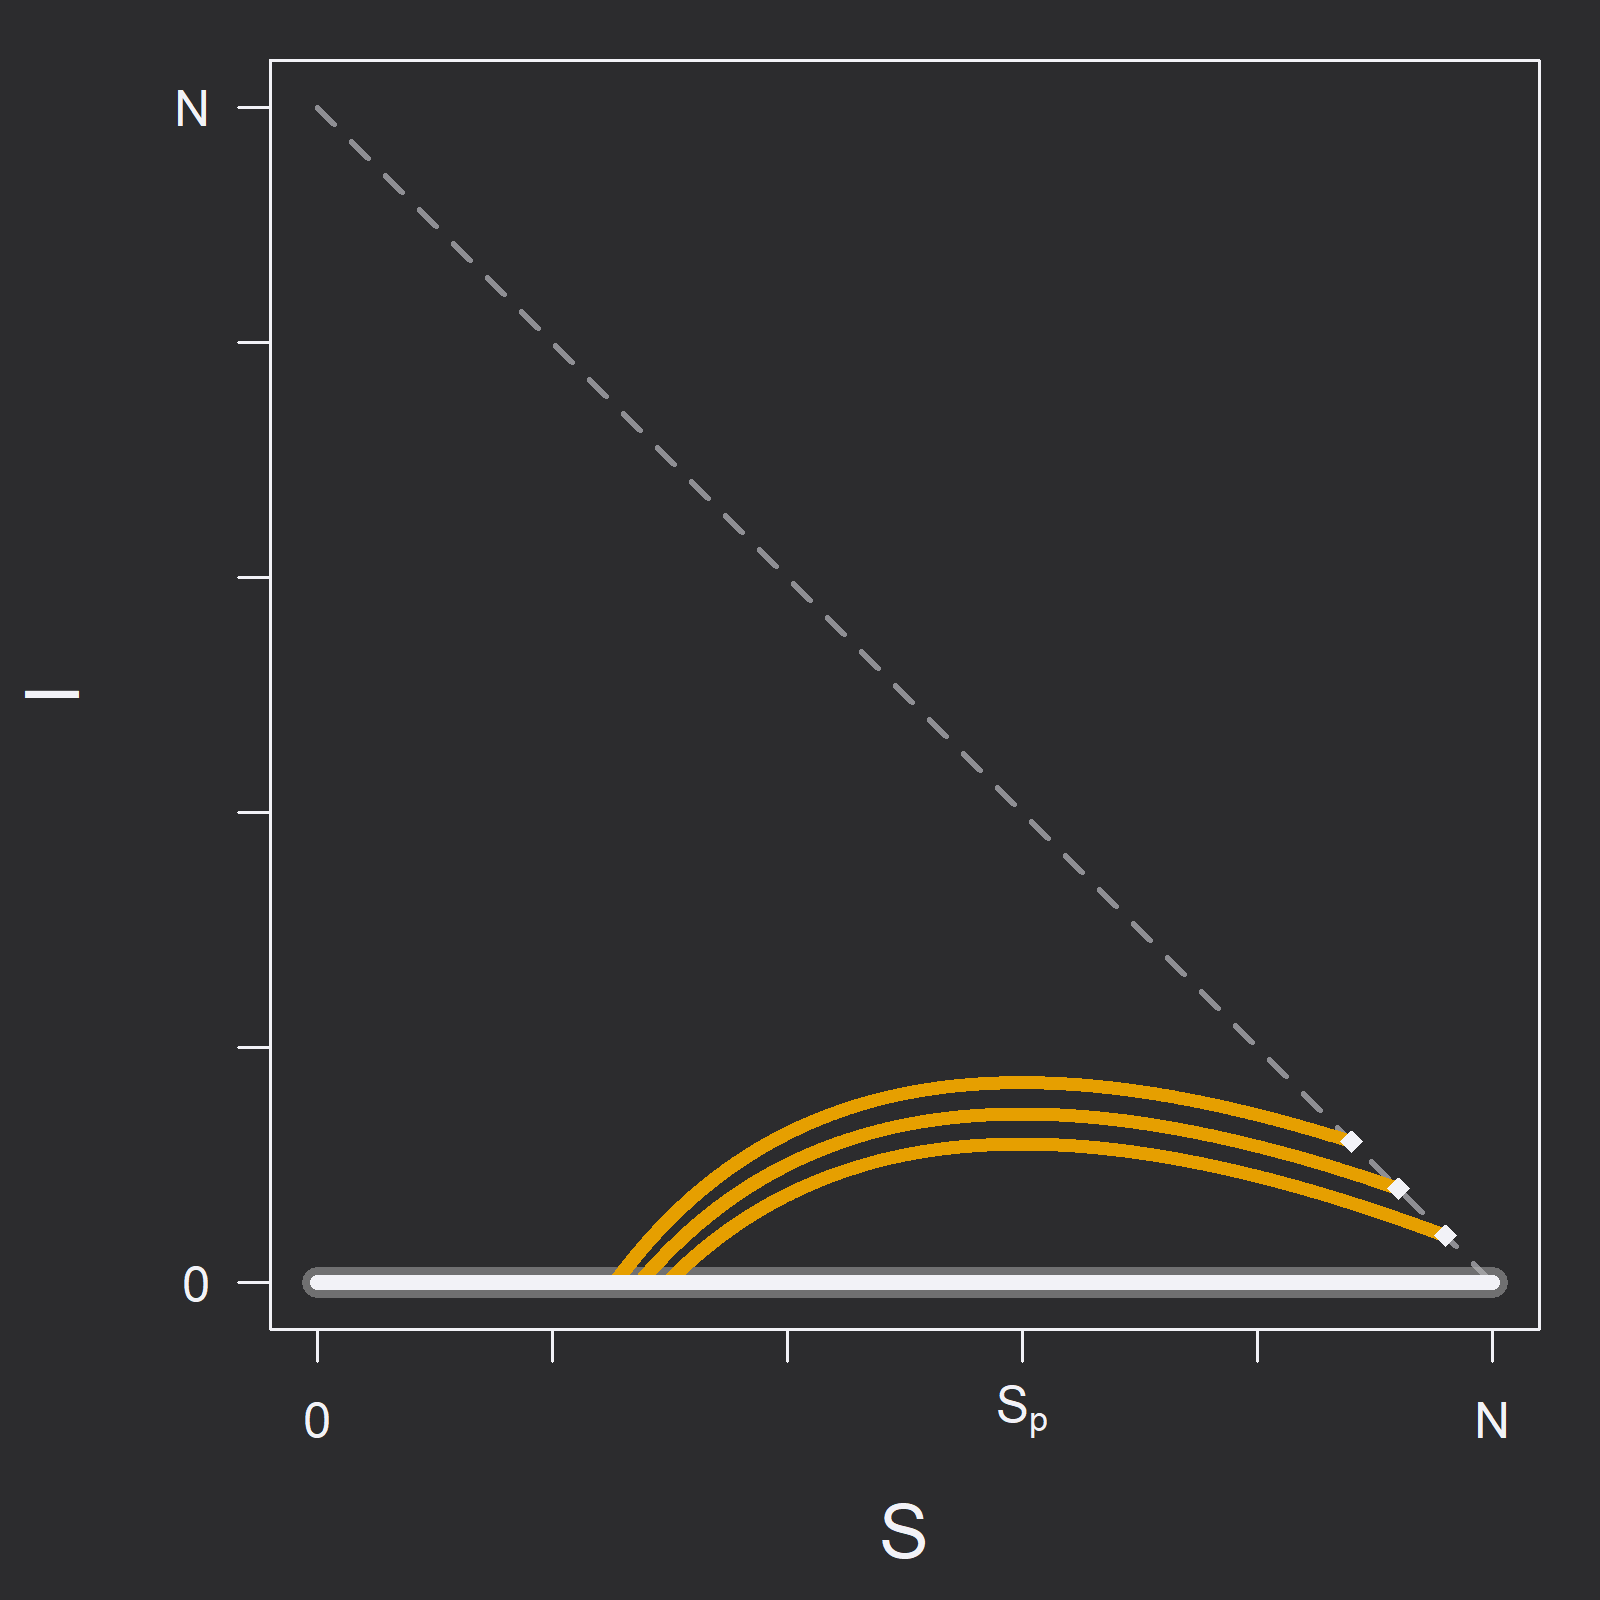
\includegraphics[width = 0.32\textwidth]{images/peak04.png} 
    
    \vspace{-1.75em}
    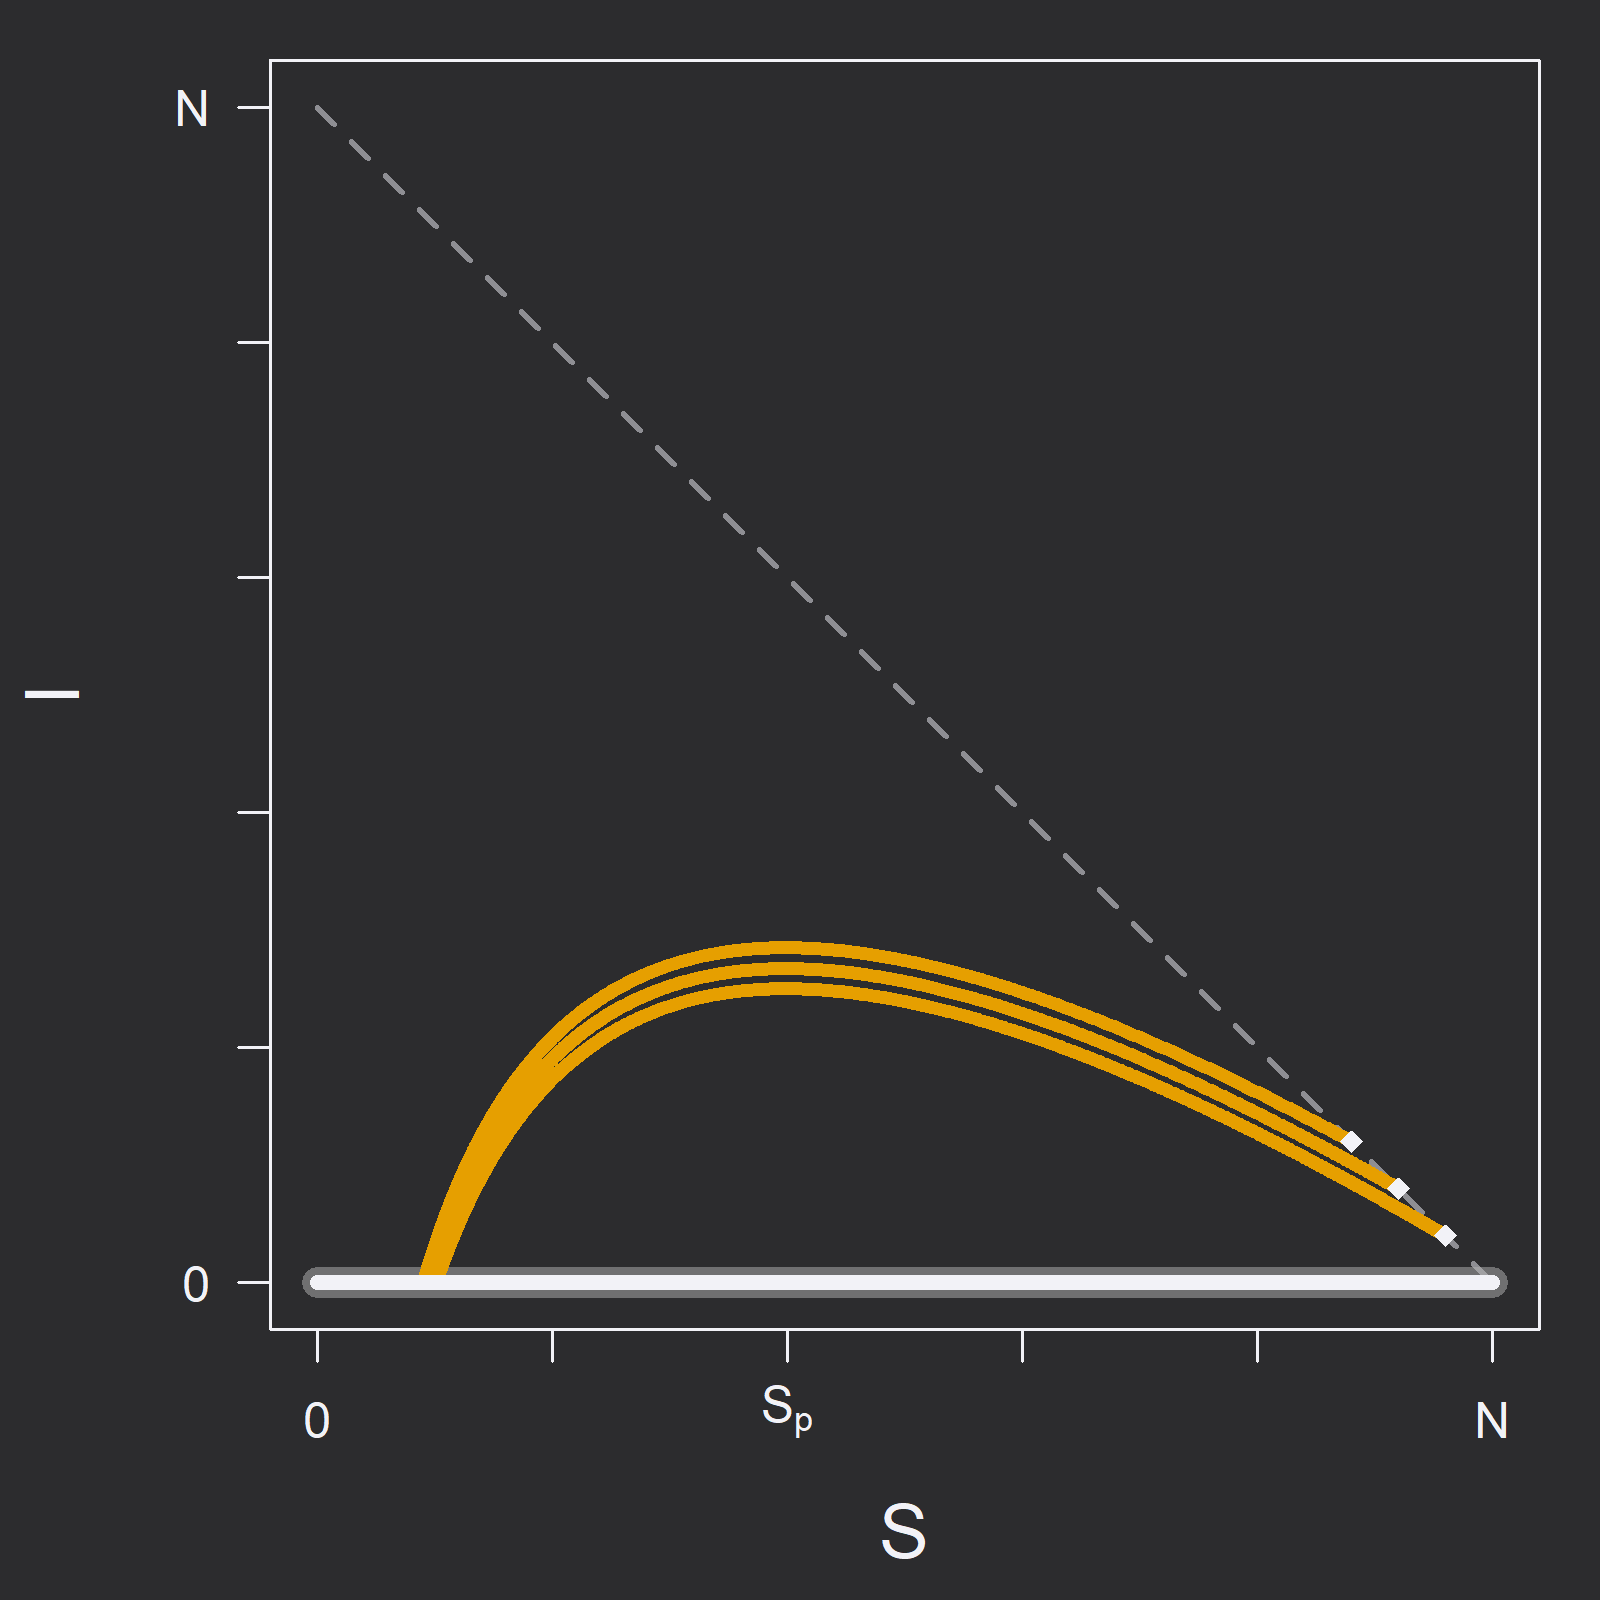
\includegraphics[width = 0.32\textwidth]{images/peak03.png} \hfill
    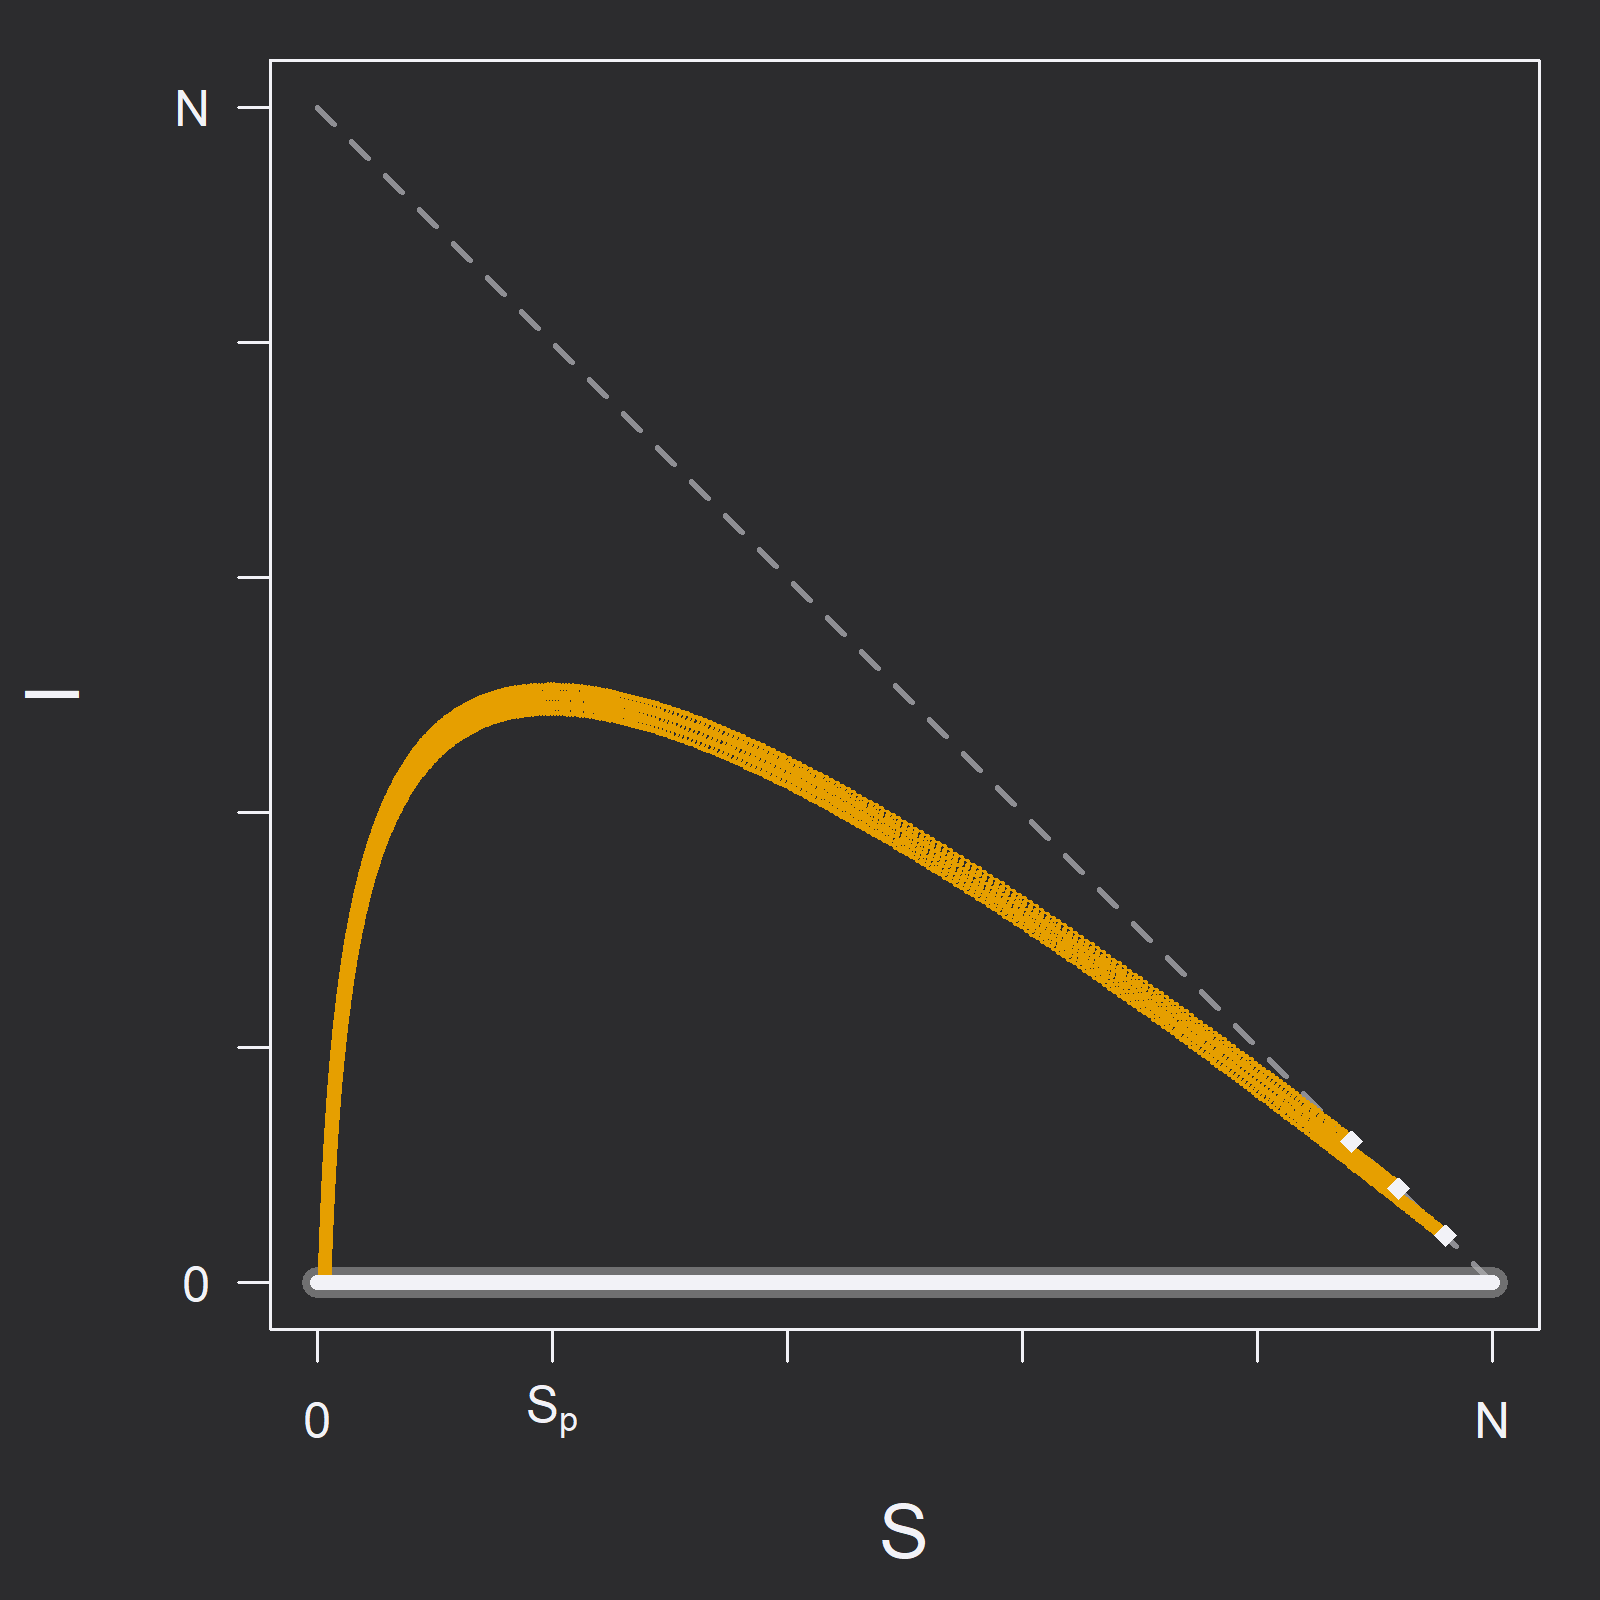
\includegraphics[width = 0.32\textwidth]{images/peak02.png} \hfill
    
\includegraphics[width = 0.32\textwidth]{images/peak01.png}
\end{figure}


    
\end{frame}



\begin{frame}{Bifurcation (?)}

\onslide<1->{
\mydark<5->{Conclusions from analyzing $\mathcal{R}_0 = \beta / \gamma$:}
}

\myskip
\begin{itemize}
    \item<2-> \mydark<6>{$\mathcal{R}_0 > 1$ $\to$ a more serious epidemic.}
    \item<3-> \mydark<5>{$\mathcal{R}_0 < 1$ $\to$ a less serious epidemic.}
\end{itemize}

\onslide<4->{
\mydark<5->{Relating this to our model parameters $\beta$ and $\gamma$:}
}

\myskip
\begin{itemize}
    \item<5-> \mydark<6>{$\beta > \gamma$ $\to$ a more serious epidemic.}
    \item<6-> $\beta < \gamma$ $\to$ a less serious epidemic.
\end{itemize}
    
\end{frame}



\begin{frame}{Social distancing}

\only<1>{
Our original model,
\begin{align*}
    \frac{\mathrm{d}S}{\mathrm{d}t} &= - \frac{\beta SI}{N} \\[1.5ex]
    \frac{\mathrm{d}I}{\mathrm{d}t} &= \frac{\beta SI}{N} - \gamma I,
\end{align*}
assumed that no changes in social behavior would occur. 
}

\only<2>{
\mydark<2>{Our original model,
\begin{align*}
    \frac{\mathrm{d}S}{\mathrm{d}t} &= - \frac{\beta SI}{N} \myhila<2>{\left( 1 - \frac{I + R}{N} \right)^k}{mycol04} \\[1.5ex]
    \frac{\mathrm{d}I}{\mathrm{d}t} &= \frac{\beta SI}{N} \myhila<2>{\left( 1 - \frac{I + R}{N} \right)^k}{mycol04} - \gamma I,
\end{align*}
assumed that no changes in social behavior would occur.} 
}

\only<3>{
\mydark<3->{Our original model,
\begin{align*}
    \frac{\mathrm{d}S}{\mathrm{d}t} &= - \frac{\beta SI}{N} \left( 1 - \frac{I + R}{N} \right)^{\myhila<3>{k}{mycol04}} \\[1.5ex]
    \frac{\mathrm{d}I}{\mathrm{d}t} &= \frac{\beta SI}{N} \left( 1 - \frac{I + R}{N} \right)^{\myhila<3>{k}{mycol04}} - \gamma I,
\end{align*}
assumed that no changes in social behavior would occur.} 
}

\onslide<2->{
We can add a \myhila<2>{\textit{social distancing term}}{mycol04} to the equations.
}

\onslide<3->{
\myhila<3>{$k$}{mycol04}~$\ge 0$ is a \myhila<3>{behavior parameter}{mycol04}.
\myskip
\begin{itemize}
    \item $k = 0$ is the original SIR model with no social distancing.
    \item As $k$ increases, society becomes more sensitive to the prevalence of the epidemic.
\end{itemize}
}
    
\end{frame}



\begin{frame}{Nullclines and equilibria (again)}

\onslide<1->{
It can be shown that 
\begin{align*}
    \frac{\mathrm{d}S}{\mathrm{d}t} &= - \beta I \left( \frac{S}{N} \right)^{k + 1} \\[1.5ex]
    \frac{\mathrm{d}I}{\mathrm{d}t} &=  \gamma I \left( \mathcal{R}_0 \left( \frac{S}{N} \right)^{k+1} - 1 \right).
\end{align*}
}

\onslide<2->{
We still have \myhila<2>{$I = 0$}{mycol04} as the line of equilibrium points.
}

\onslide<3->{
However, the point of maximum infections $S_p$ is now given by
\begin{align*}
    S_p = \frac{N}{\mathcal{R}_0^{1/(k+1)}}.
\end{align*}
}
    
\end{frame}



\begin{frame}{Effect of increasing $k$}

\onslide<1->{
We can see that 
\begin{align*}
    \lim_{k \to \infty} S_p = \lim_{k \to \infty} \frac{N}{\mathcal{R}_0^{1/(k+1)}} = N.
\end{align*}
}

\onslide<2->{
In the case of $\mathcal{R}_0 > 1$, as $k$ increases, the peak will be pushed to the right.
}

\onslide<3->{
As a result, \myhila<3>{\textit{the epidemic will not be as severe}}{mycol04}.
}
    
\end{frame}



\begin{frame}{Effect of changing $k$}

\begin{figure}
    \centering
    \onslide<1->{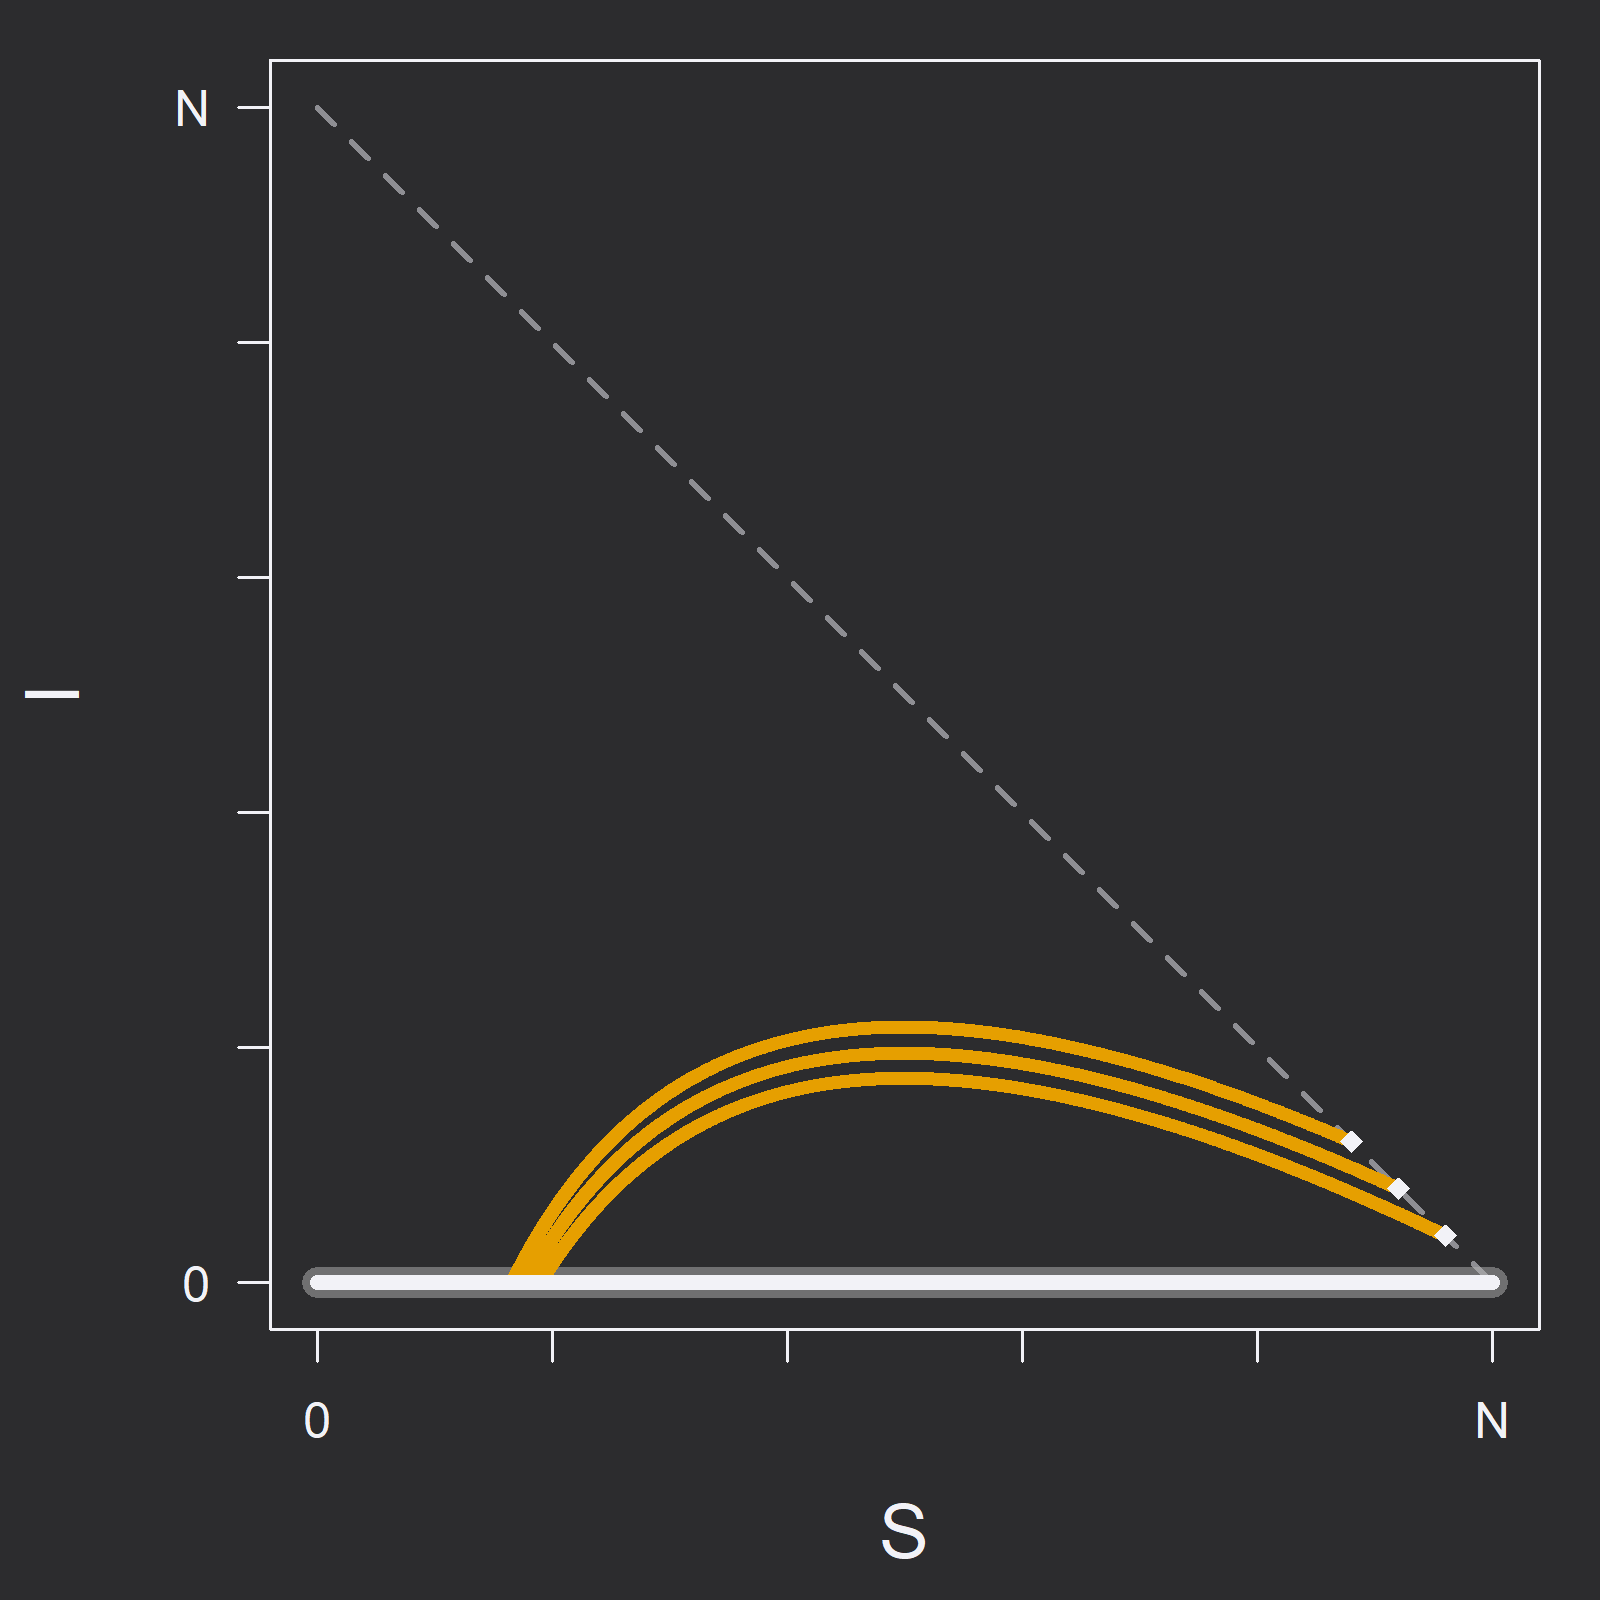
\includegraphics[width = 0.32\textwidth]{images/basic.png}} \hfill
    \onslide<2->{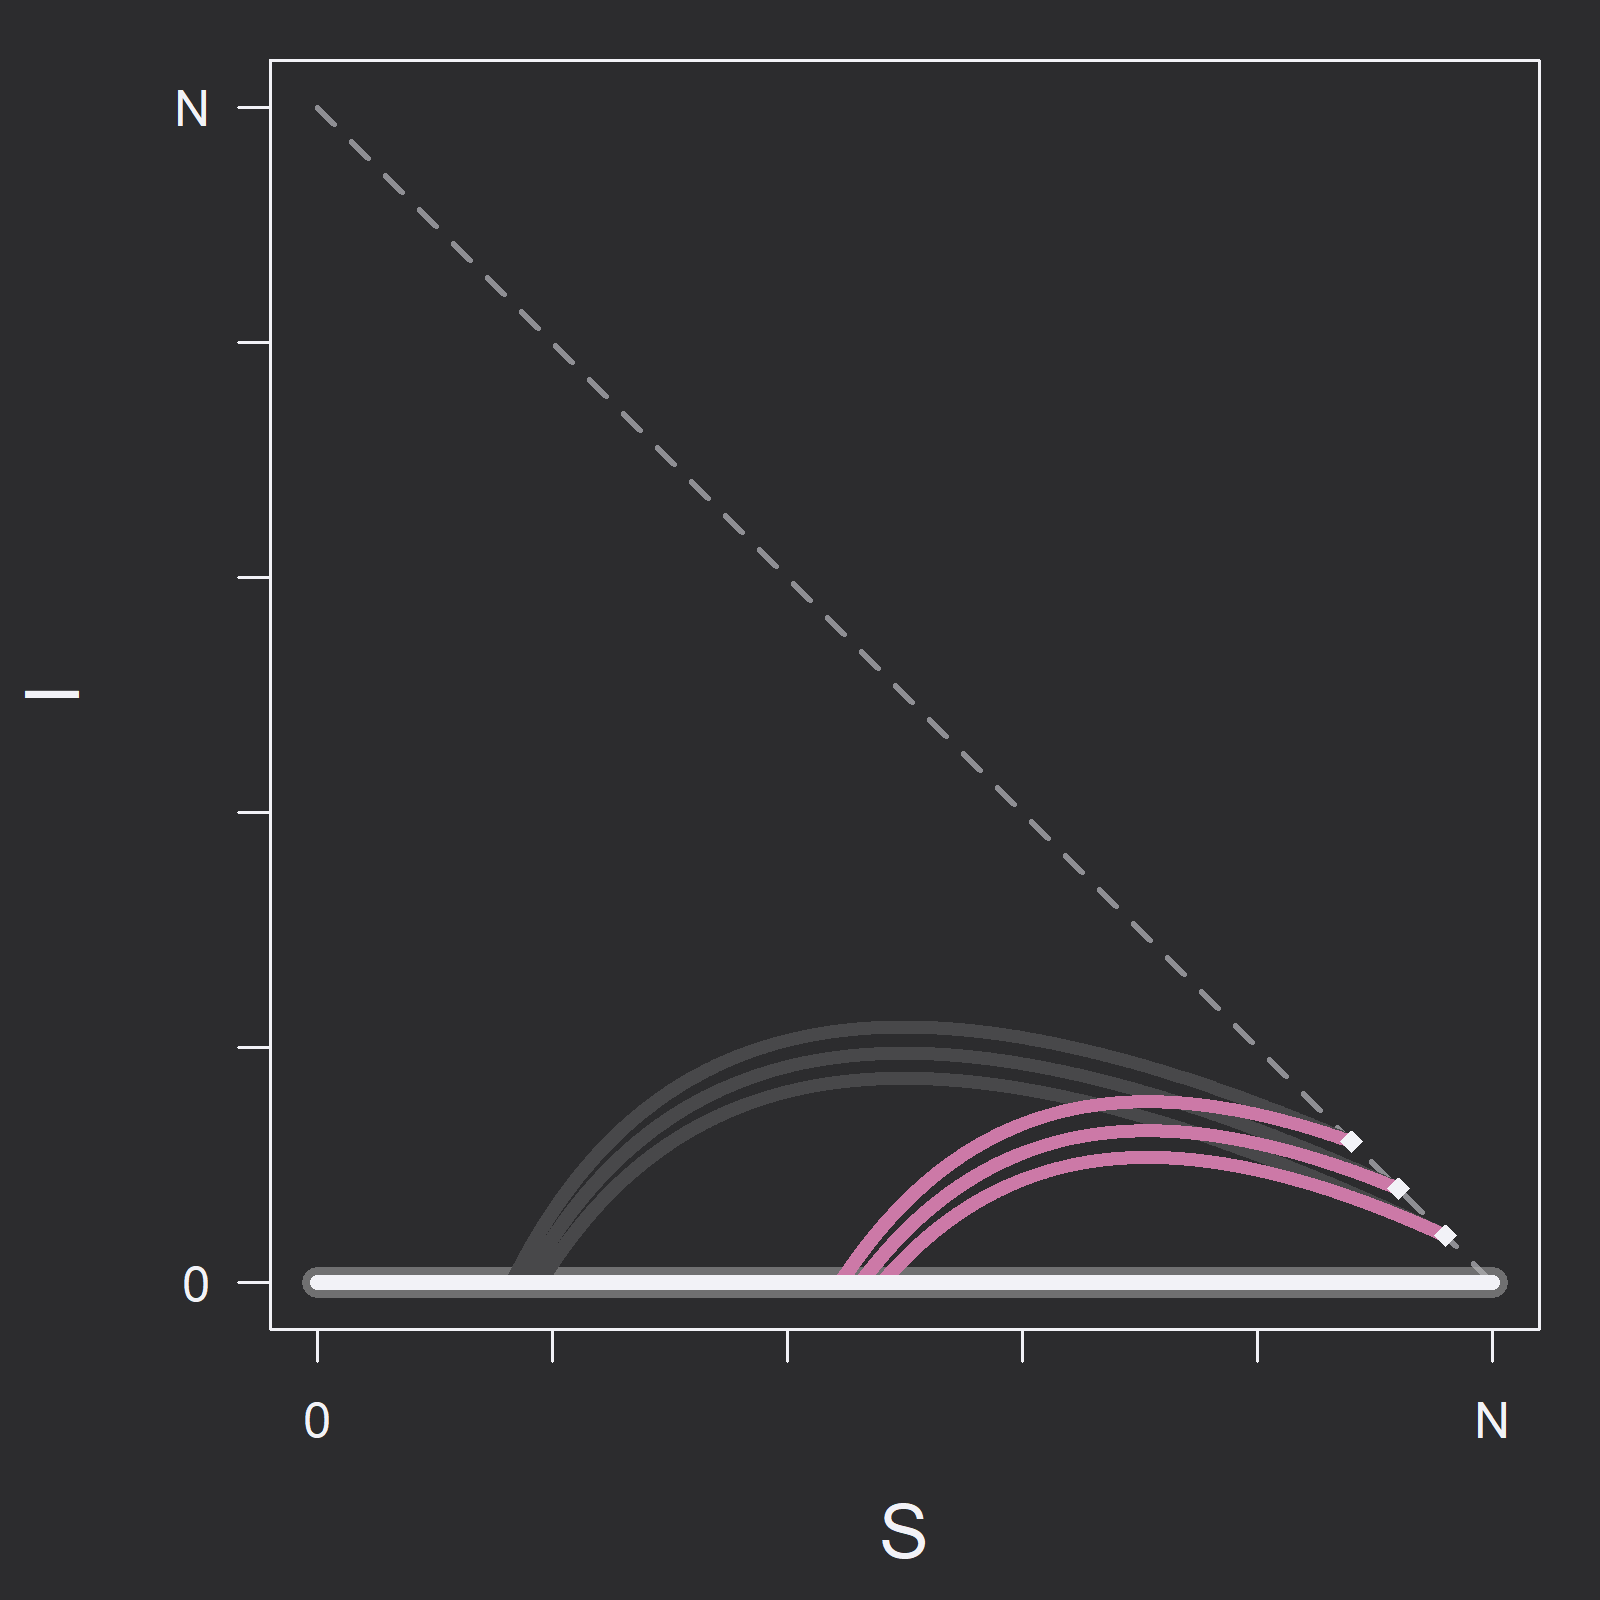
\includegraphics[width = 0.32\textwidth]{images/comp_linear.png}} \hfill
    \onslide<3->{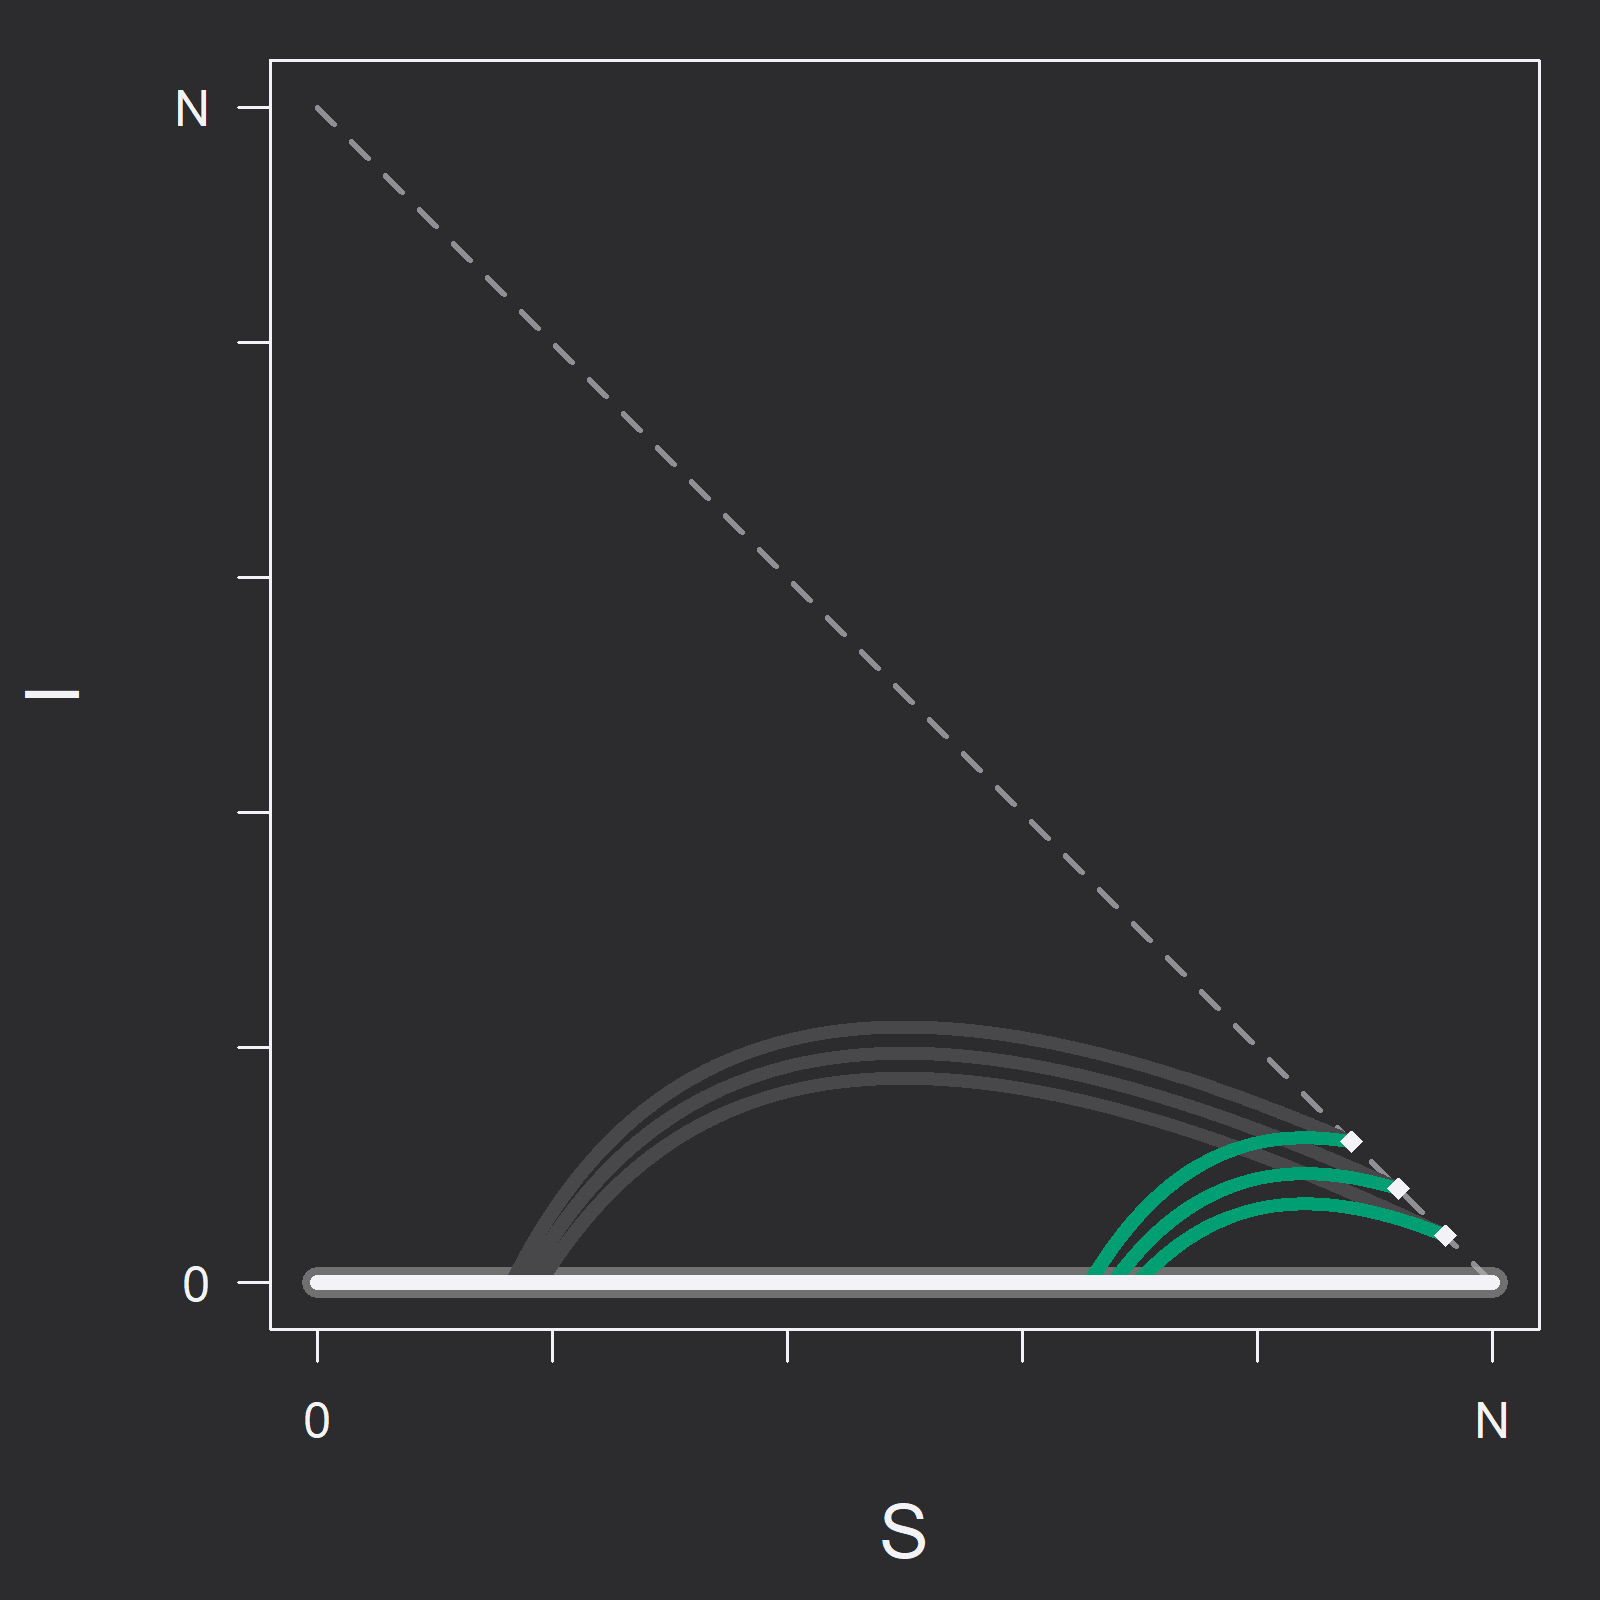
\includegraphics[width = 0.32\textwidth]{images/comp_nlinear.png}}
\end{figure}

\myskip
\onslide<1->{
\mydark<2->{The left panel shows when \myhila<1>{$k = 0$}{mycol01} $\to$ no social distancing.}
}

\myskip
\onslide<2->{
\mydark<3->{The middle panel shows when \myhila<2>{$k = 1$}{mycol05} $\to$ moderate social distancing.}
}

\myskip
\onslide<3->{
The right panel shows when \myhila<3>{$k = 3$}{mycol03} $\to$ aggressive social distancing.
}
    
\end{frame}



\begin{frame}{Population affected}

\onslide<1->{
The \mydef{percent of population affected} is given by $(I + R)/N$. 
}

\myskip
\begin{itemize}
    \item<2-> We can model how this value changes over time.
\end{itemize}

\begin{columns}

\begin{column}{0.45\textwidth}

\begin{figure}
    \centering
    \onslide<3->{
\includegraphics[width = 1.0\textwidth]{images/affect01.png}}
\end{figure}

\end{column}

%\hfill

\begin{column}{0.45\textwidth}

%\begin{itemize}
%    \item<4-> \myhila<4->{$k = 0$}{mycol01}
%    \item<4-> \myhila<4->{$k = 1$}{mycol05}
%    \item<4-> \myhila<4->{$k = 3$}{mycol03}
%\end{itemize}

\onslide<4->{
Things to notice:
}

\vspace{1em}
\begin{itemize}
    \item<5-> Long term: social distancing has huge affect.
    \item<6-> Initially, percent affected looks \myhila<6>{\textit<6>{very similar}}{mycol04} between the three models.
    \item<7-> This shows pitfall of not accounting for changes in social behavior.
\end{itemize}

\end{column}

\hfill

\end{columns}
    
\end{frame}



%\begin{frame}{Key takeaways}

%\onslide<1->{
%Social distancing works
%}
    
%\end{frame}

\end{document}
